\section{The Bayesian Method}
\label{inference_methodology}

\subsection{Income Homophily}

\begin{figure}[ht]
	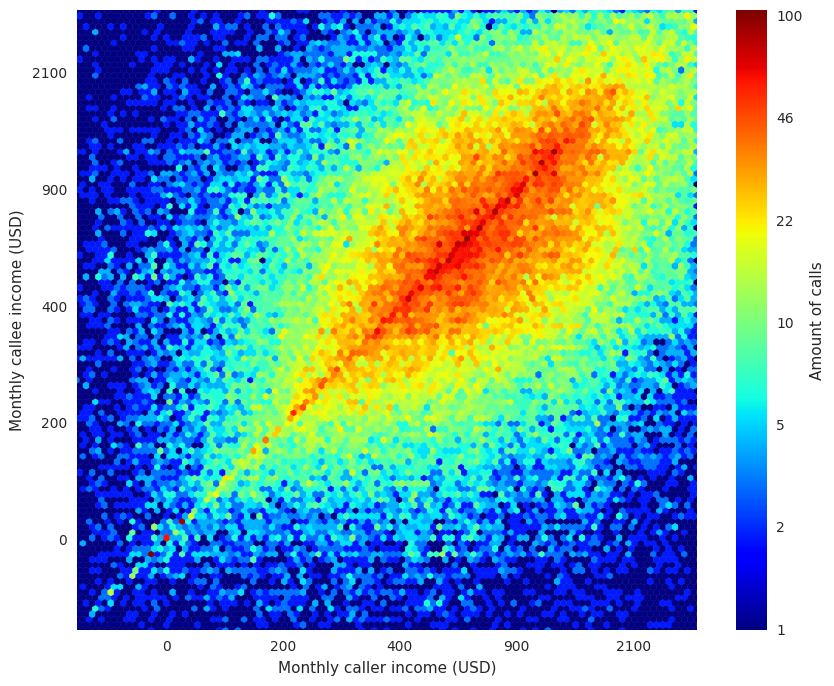
\includegraphics[width=\columnwidth]{Homophily_income_origin_target_usd.png}
	\caption{Heatmap showing the number of calls between users, according to their monthly income. There is a higher probability that the callee and the caller have similar income levels.}
\label{homophily_heatmap}
\end{figure}

The main contribution of this work is the estimation of the income of the telco users for which we lack banking data, but have bank clients in their neighborhood of the network graph. To show the feasibility of this task, we first show the existence of a strong income homophily in the telco graph as is evidenced in \Cref{homophily_heatmap}.

For each pair $\left< o, d \right> \in \mathlarger{G}$, we define $X$ as the set of incomes for callers and $Y$ as the set of incomes for callees. According to what we can observe in \Cref{homophily_heatmap}, $X$ and $Y$ should be significantly correlated. Given the broad non-Gaussian distribution of the income's values, we choose to use a rank-based measure of correlation which is robust to outliers.

Namely we computed the \textit{Spearman's rank correlation} defined in \cref{spearman} to test the statistical dependence of sets $X$ and $Y$. This coefficient gives us a correlation coefficient of $\mathbf{r_s = 0.474}$. We also compared our result with a randomized null hypothesis, where links between users are selected randomly disregarding income data, obtaining a $p$-value of $p < 10^{-6}$. These values for $r_s$ and $p$ show a strong indication of income homophily among users in our communication graph. This observation is consistent with the results reported in~\cite{leo2015socioeconomic}.

\begin{equation}
r_s = \mathlarger{\rho}_{\operatorname{rank}(X) \operatorname{rank}(Y)} = \frac{\operatorname{cov}(\operatorname{rank}(x), \operatorname{rank}(y))}{\sigma_{\operatorname{rank}(X)} \sigma_{\operatorname{rank}(Y)}}
\label{spearman}
\end{equation}

We can take advantage of this homophily to propagate income information to the rest of our graph $\mathP$, where we don't know the income of all the users.

\subsection{Prediction Algorithm}

Instead of predicting the exact value of a user's income, our strategy is to distinguish between only two income categories depending on their monthly income expressed in US dollars: $R_1 = \closeopen{55}{350}$ and $R_2 = \closeopen{350}{\infty}$. These two categories represent roughly users with low or high income in the country where this study was made. We place these into two distinct groups $H_1, H_2 \subseteq G$ depending on $g_s$, the users' income: $H_1$ for poorer users, and $H_2$ for wealthier ones.

We define the set $Q$ as the group of users having at least one connection link to bank clients. For each user $q^j \in Q$, we compute the number of outgoing calls $a^j_i$ to the category $H_i$. Our hypothesis, given the observed homophily, is that if a user $q^j$ has a higher number of calls $a^j_i$ to the category $H_i$ than the other category, it would be more likely to belong to the $H_i$ income category. In other words, a person is usually in the same income category as the majority of people it calls.

A straightforward approach would be to define the income category of a user as the category where most of its contacts belong. The problem with this approach is that it does not factor in the higher uncertainty in our estimates for users with fewer calls. To address this uncertainty, instead of using calling frequencies to define the probability of a user belonging to the high income category, we use the amount of calls $a^j_i$ as parameters defining a Beta distribution for the probability of belonging to a given category. We have therefore taken a Bayesian rather than a frequentist approach to income prediction.

We define $\Beta^j$ as the Beta probability distribution function for each user, which defines a distinct distribution for each user. Having obtained the Beta distribution for the probability of belonging to the high income category, we then find the lowest 5\textsuperscript{th} percentile $p_{\operatorname{lower}}$ for this probability. If $p_{\operatorname{lower}}$ is above a given threshold $\tau$, we set the user's income to $H_2$, otherwise we set his income category to $H_1$. We note that this criteria takes into account both the mean and the broadness (uncertainty) of the distribution. We also note that the category assigned to a user depends not only on its Beta distribution but also on our choice of $\tau$.

%We therefore choose a value for $\tau$ which maximizes the trade off between true positive ($TPR$) and false positive ($FPR$) rates: $TPR=TP/P$ and $FPR=FP/N$ where $TP$ is the number of correctly predicted users with high income, $P$ is the total number of users with high income, $FP$ is the number of users incorrectly classified as having high income, and $N$ is the total number of users with low income.

%For each user $q^j$ we estimate and the corresIn this way we obtained a Dirichlet distribution for each user $q^j$ and compute

%According to the Dirichlet Distibution, each user has a caller income category probability density function of the form

%For all the other users in the telco having at least one link to any other telco user with a defined income $q \in Q = \left\{x \in \left( N \setminus B \right) \mid (\exists y \in G) \left< x, y \right> \in P \vee \left< y, x \right> \in P \right\}$, we can use this distribution to infer the probabilities of being part of each group $H_1, \ldots, H_5$, and this way approximate the economic status.
